\section{Introduction}

Cyber-physical systems (CPSs) can be difficult to design due to the heterogeneous 
nature of the domains in which they must operate.  Safety-critical control applications also 
require a level of formal verification, to prove to certification authorities (and 
therefore indirectly to the consuming public) that use of these devices entails only 
minimal danger.  

%Model-based design and analysis tools help system
%designers assess performance, stability, schedulability, and a host of other
%important properties.  
Modern control design and embedded development approaches incorporate code
synthesis techniques as well as integrating analysis tools into a model-based 
design flow. Each of these designs, assessments, or generations are
typically made independently by analysts trained in either an engineering domain
(mechanical, electrical, or control design) or in computer science
(schedulability, componentization, or deployment concerns).
Artifact generation from models occurs at different stages of the design
process: generating functional code, analysis models, and possibly platform
specific wrapper code and configuration.  Each analysis tool may
have its own modeling language with distinct semantics. Semantic differences can
lead to inconsistencies in the understanding of the design, so details must be
kept consistent across design specialization domains and between model
interpretation stages.

In current practice, much of the reconciliation of design discrepancies is still
done by hand.  Individal designers or review teams discover design
inconsistencies.  Manual reconciliation of issues occurs as individual
designers receive assignments to modify and correct the design.  Several large
modeling tool projects (for example, AADL \cite{modeling:aadl_control_systems}
and Topcased\cite{tools:Topcased}) work to integrate tools from
independent research and development teams into a common design environment
featuring a standardized modeling language.  Resolution of semantic consistency
between tools is a serious issue in such efforts.

Supporting such heterogeneity of analysis tools and domains requires everyone involved in 
the design process to have a consistent view of design details.  Reconciling semantics 
between formalisms and tools is costly and time-consuming.  Often the effort can not be 
justified outside of academic research unless the results are applicable to numerous designs.

%\begin{figure}
%\centering
%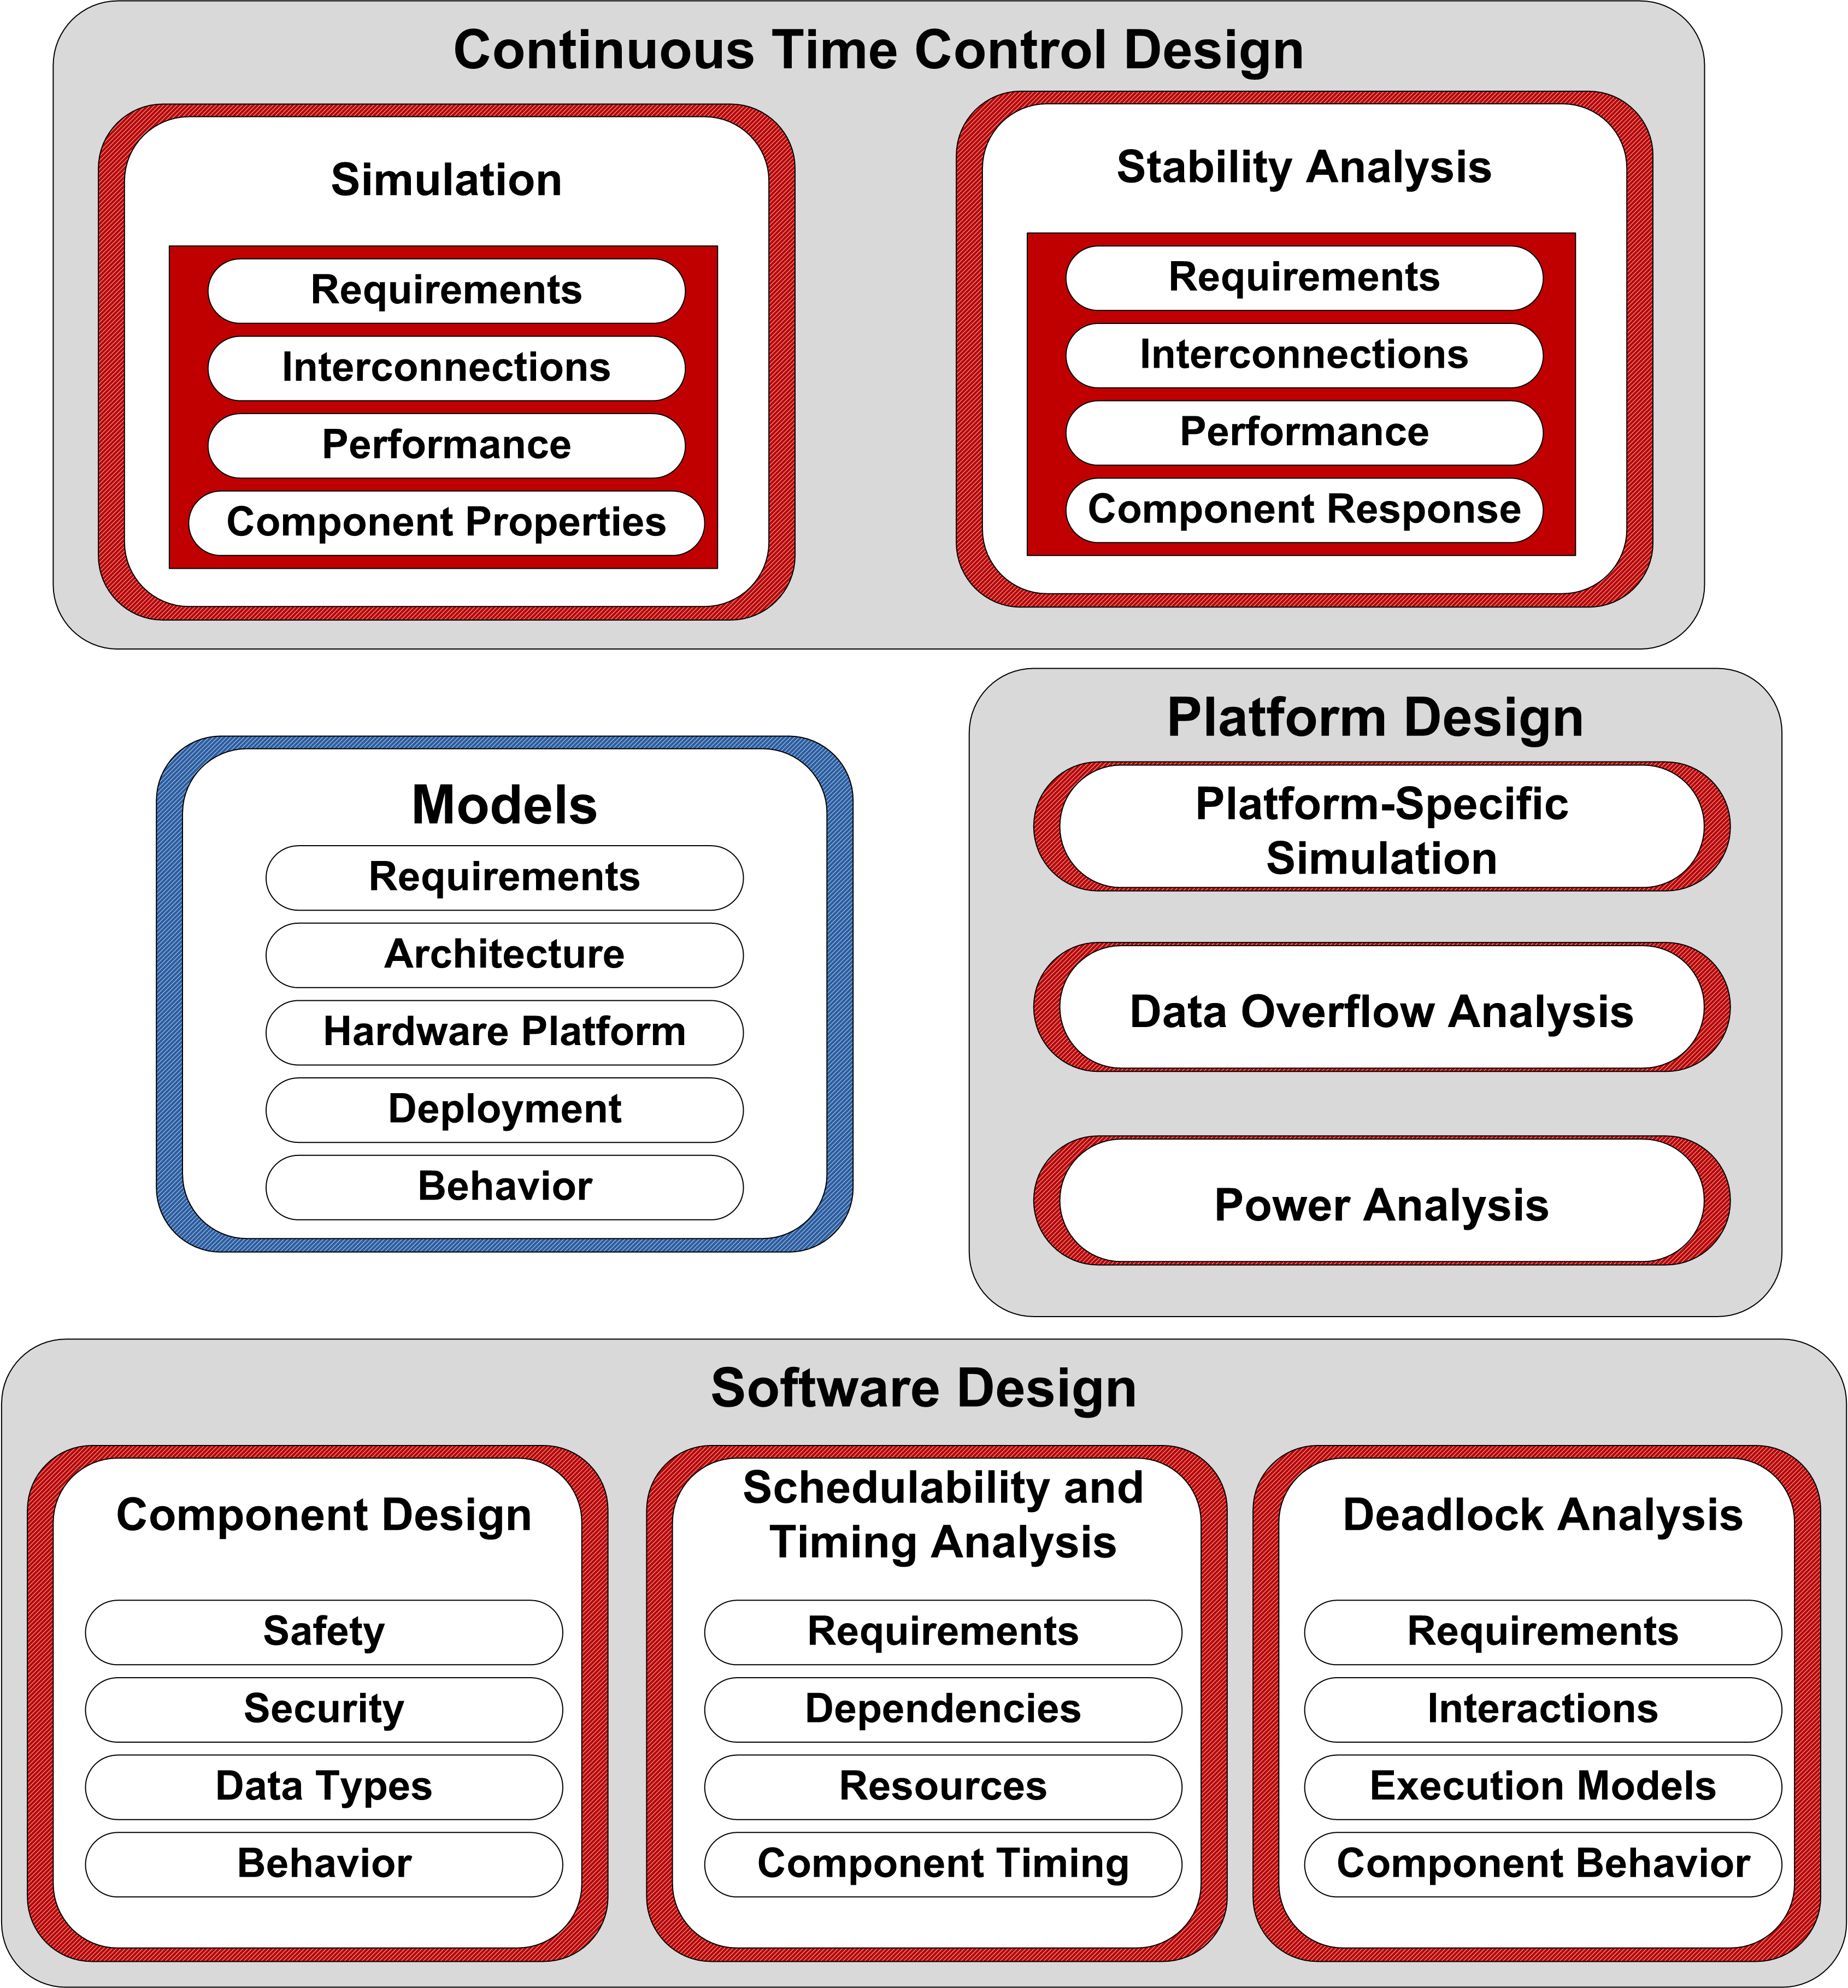
\includegraphics[width=0.72\columnwidth]{figures/analysis_integration.png}
%    \caption{Conceptual illustration of the many facets of a model-based CPS design process. 
%Reconciling the detils of all of these semantic models is a significant challenge. 
%Tools must not only address details between them, but support realistic work flows for development teams.}
%    \label{fig:integration}
%\end{figure}

In the model integrated computing approach, domain specific modeling languages represent 
different aspects of the design, with the promise of consistently integrating different tools 
and techniques.  We present here a sketch of a formal model-based approach which promises to tame 
many of the difficulties involved in consistently integrating heterogeneous analysis tools into a 
single workflow.  Our approach can be considered as an implementation of the tool integration ideas 
in \cite{modeling:hybrid_abs}, but with variations of the details included in the design language.  
Specifically we propose the following main ideas:

\begin{enumerate}

\item A front end graphical modeling language which integrates into existing design 
workflows\cite{modeling:aces08}.

\item A single transformation from front end models to an intermediate language explicitly 
representing a flattened semantic model, including parameters and objects to imply a precise 
behavioral semantics.  We differ from the approach in \cite{modeling:hybrid_abs} by abstracting the dynamic component interface behavior using passive control design 
techniques. We rely on the resulting robustness and compositionality of the passive approach 
to simplify design analysis and implementation, as our design language is
specific to distributed embedded control systems.  Note that we only have preliminary 
support for passive control design and analysis -- this is a work in progress (see \cite{ncs:mic} 
for preliminary work in this area).

\item Both the front-end and intermediate languages support platform-based design \cite{modeling:platform}, 
separating component-level concerns and interaction concerns where possible.  The platform for this
language is the time-triggered architecture\cite{timed:tta}, and the tool suite supports deployment
to a time-triggered execution environment\cite{timed:frodo} in order to preserve synchronous execution
semantics.

\item Generation of analysis models and code from the intermediate language
using simple template generation techniques\cite{sched:analysis}.

\item Representation of structural and behavioral concepts from the intersection of the semantic 
domains of integrated tools as primitives in the front end language.

\item Round-trip incorporation of calculated analysis results into the modeling environment to 
maintain consistency as models pass between design phases.

\end{enumerate}

The described approach is part of the ESMoL modeling language and software design 
suite\cite{modeling:aces08}.  ESMoL is a research experiment in the implementation of modeling 
tools to support compositional analysis and design frameworks.  In our design flow a modeler 
imports Simulink/Stateflow models \cite{tools:mathworks} into the ESMoL language, adds architecture 
elements, platform design, and deployment concepts, then performs automated analysis and synthesizes 
code for execution on a time-triggered platform.  We aim to support iterative
development, as analysis data can flow back to earlier stages for re-design or
re-evaluation.  The language and tools also include preliminary support for
requirements modeling, by allowing specification of maximal latency 
bounds between computational tasks in the design. Table
\ref{tab:consistencyTools} gives an overview of our toolchain design goals and
philosophy, considering details from three different semantic models.

Our tools enforce a single view of the interpretation of design details in a
design model. Consistency is required in both the structure of the design models
(i.e. the componentization and its relations) as well as the behavior
represented by the design models (i.e. the model of computation in which tasks
are executed and their behavior within that model). 

\begin{figure}
\centering
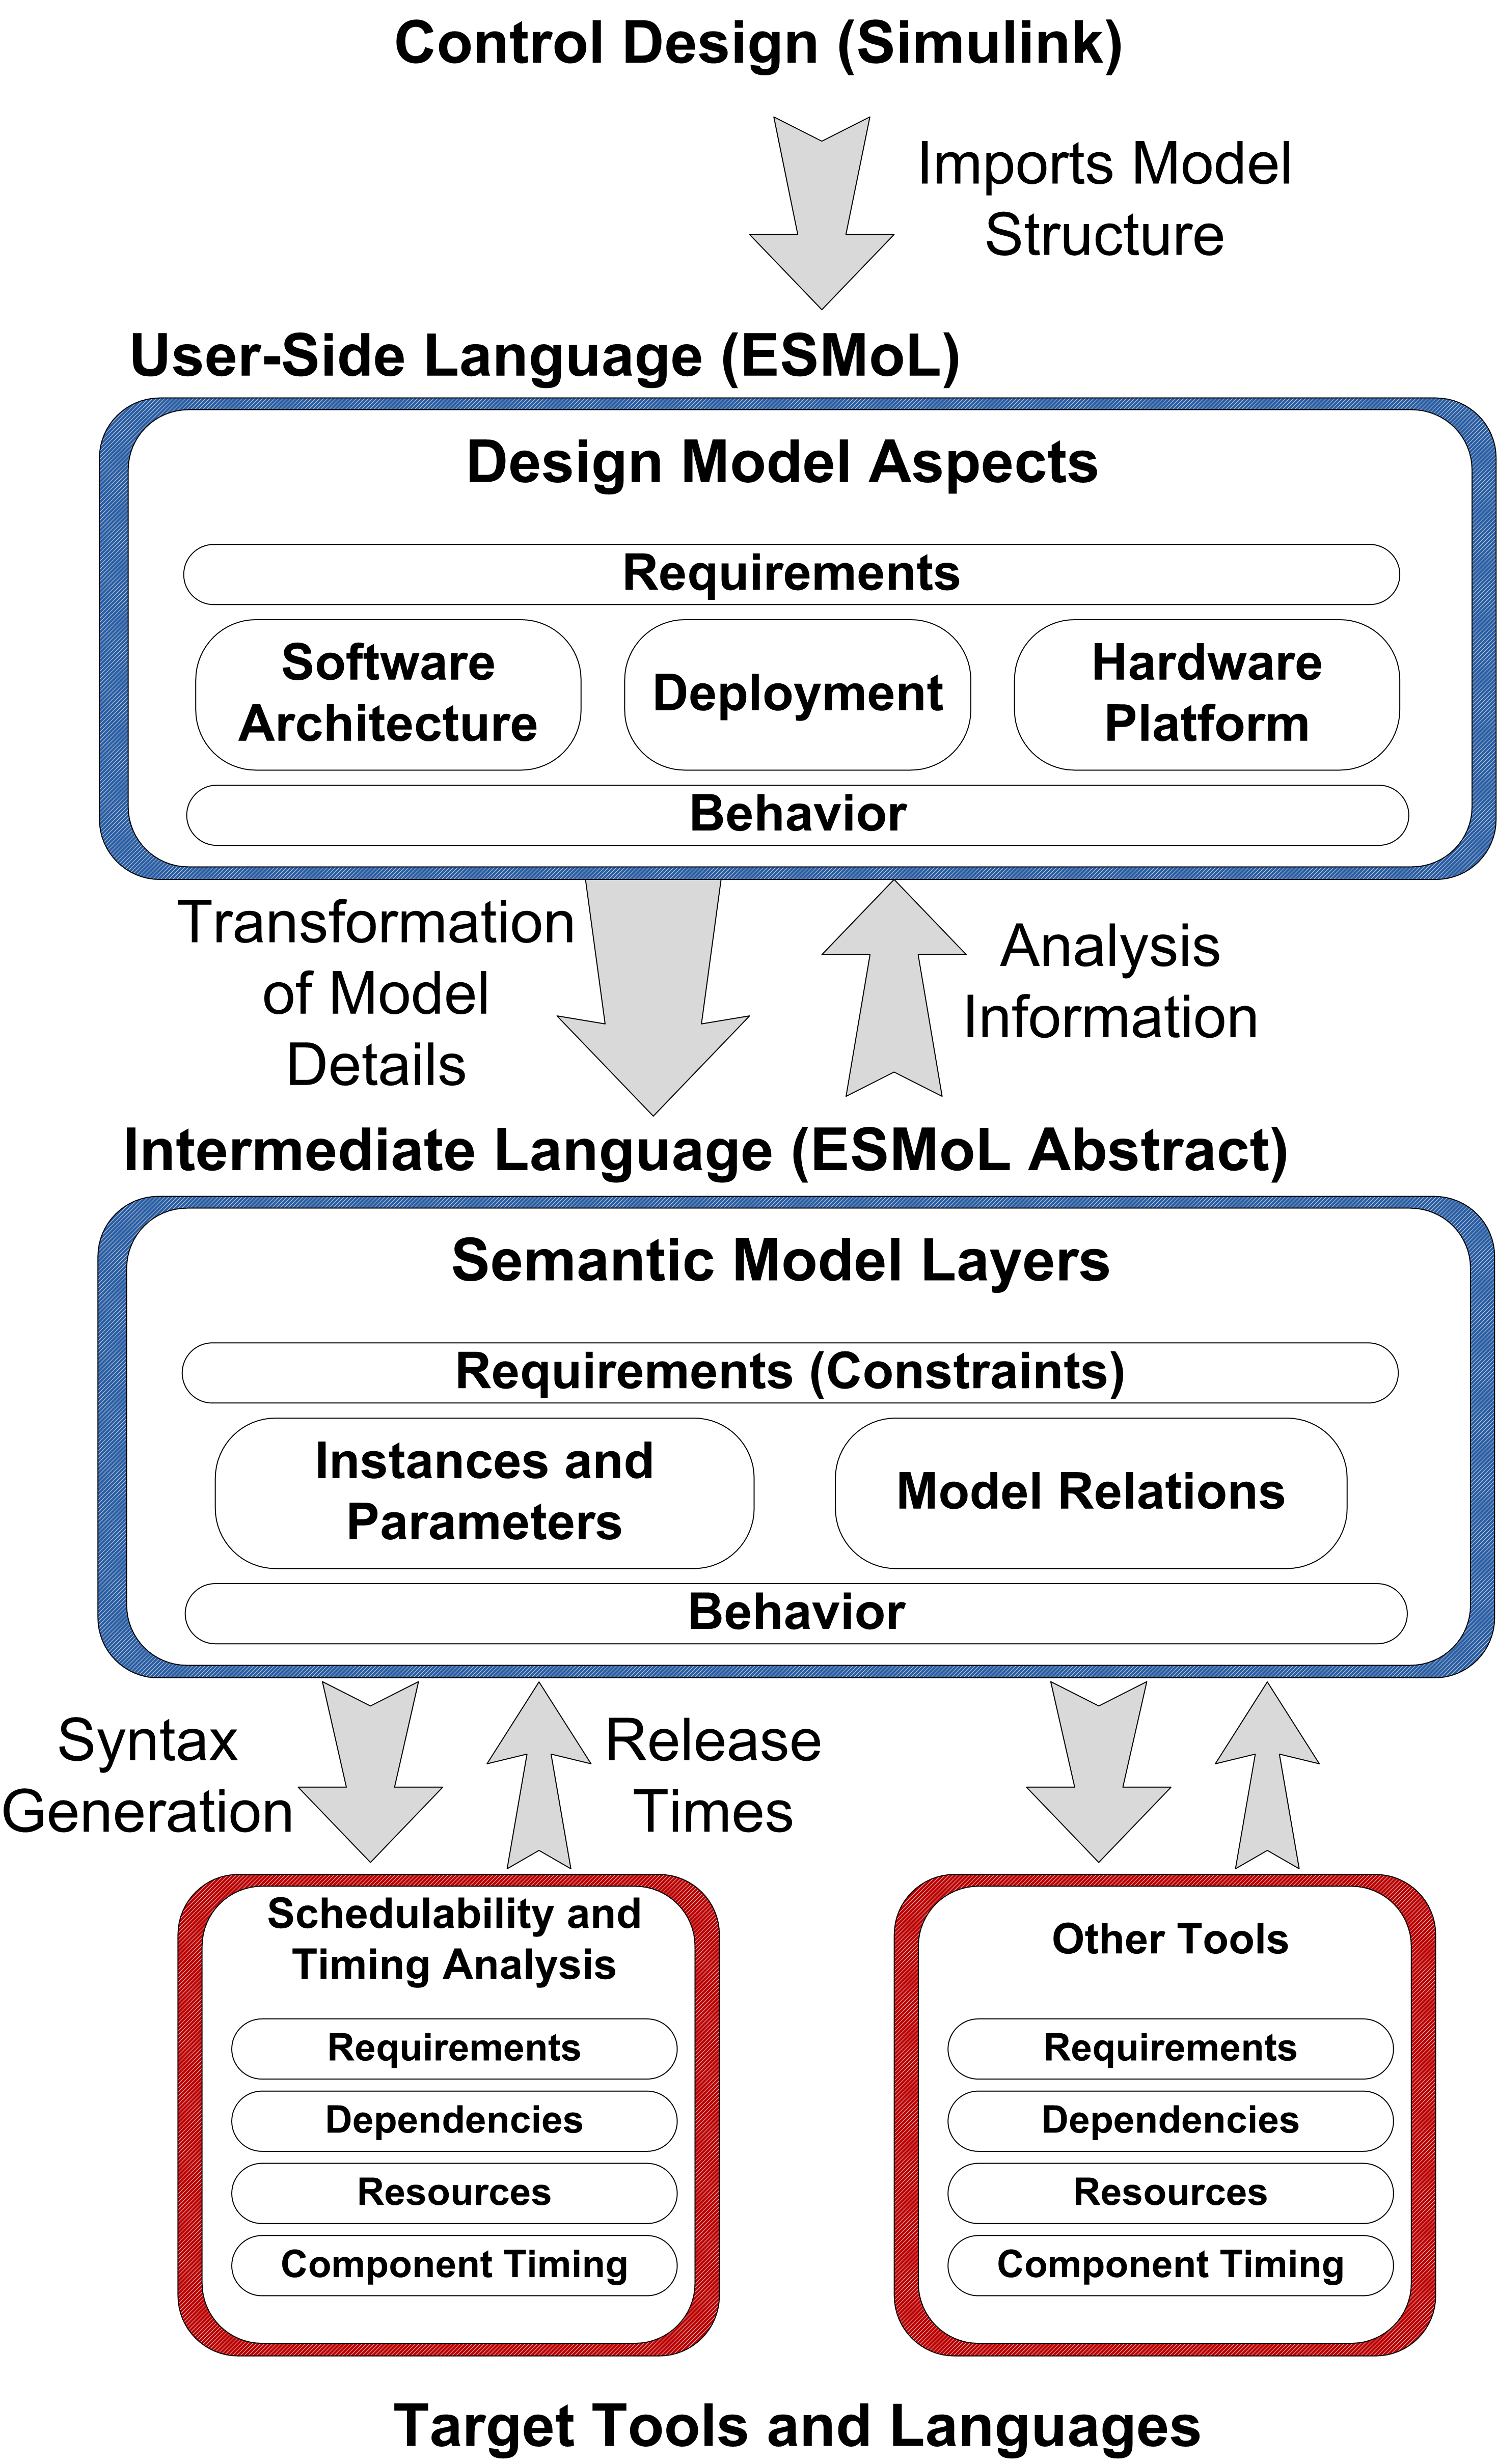
\includegraphics[width=0.5\columnwidth]{figures/designflow.png}
    \caption{Suggested flow of design models between design phases. During
design iterations, analysis data can be transformed and fed back to designers. }
    \label{fig:designflow}
\end{figure}

The model-integrated computing approach (MIC) \cite{mic:overview} facilitates
the essential part of the consistency effort.  Figure \ref{fig:designflow} depicts
a design flow that includes a user-facing modeling language for design and a
language for explicit representation of semantics.  In the Generic Modeling
Environment (GME) \cite{mic:gme} a designer creates a 
software design from an imported Simulink control design.  Rather than designing
a user-friendly graphical modeling language and directly attaching translators
to analysis tools, we created a simpler abstract intermediate language whose
elements are similar to those of the user language. The first model
transformation flattens the user model into the abstract intermediate form,
translating parameters and resolving special cases as needed. Generators for code 
and analysis are attached to the abstract modeling layer, so the second-stage
transformations are simpler, and are isolated from changes to the user language.

\begin{table}[htb]
	\centering
		\begin{tabular}[width=0.75\columnwidth]{@{\extracolsep{\fill}} |
p{1.7cm} | p{4.6cm} | p{4.6cm} | }
		\hline
		\multicolumn{3}{|c|}{Behavioral Consistency Goals} \\
		\hline
		. & Execution Order Constraints & Timing Constraints \\ \hline \hline
		Dynamic Stability (Comp) & Passive controllers run synchronously at a fixed rate determined by control analysis and simulation. & Control functions execute in bounded time, measured for the given platform. Nominal sample rates are passive and stable. \\ \hline
		Dynamic Stability (Intr) & Passive control design decreases the effects of delays from scheduling and platform timing jitter. Maximum acceptable sample delay is one possible abstraction for these effects. & Timing guarantees are not yet considered in our passive control design framework. \\ \hline
		\hline
		Scheduling (Comp) & We use a synchronous execution model to precompute component invocation order within tasks to eliminate local data hazards. & Each task has a known, bounded execution time (WCET/Deadline parameters are in the model).  \\ \hline
		Scheduling (Intr) & Message and task dependencies are translated to linear constraints, along with constraints to model resource utilization. & Scheduling achieves the desired sample rate and enforces latency bounds between tasks.  A proposed delay abstraction could represent schedule slack, and latency could be used to budget slack. \\ \hline
 \hline
		Execution Environment (Comp) & Statically precomputed task
release times are used to configure the generated tasks, and the VM enforces
start times. & We assume bounded-time task execution.  VM tasks can not be
preempted, and so execute as quickly as possible to meet their deadline (WCET in
this case). \\ \hline
		Execution Environment (Intr) & Clocks on separate nodes are
synchronized to support synchronous execution.  Frame sync (null) messages are
sent at the start of the common hyperperiod to keep nodes executing together.  &
Time-triggered schedules prevent collisions, so messages transfer
deterministically. Measured transfer overhead is captured in the platform
design, and used in scheduling calculations. \\ \hline
		\end{tabular}
	\caption{Summary discussion of the behavioral consistency goals from the
point of view of each design stage of our tools so far.  The table covers
relationships between three different semantic models: dynamic stability,
schedulability, and deadlock freedom. The (Comp) notation refers to local
(component/task) level concerns, and (Intr) refers to design concerns at the
level of interactions between components, consistent with our platform
abstraction.  The ESMoL language constructs should embody the correct
resolution of these design issues, and maintain the assumptions through all
stages of design and execution.}
	\label{tab:consistencyTools}
\end{table}